\documentclass{article}
\usepackage{amsmath}
\usepackage{tikz}
\usepackage{graphicx}
\usepackage[lofdepth,lotdepth]{subfig}
\usepackage{makeidx}
\makeindex
\usepackage[bookmarks,colorlinks]{hyperref}
\hypersetup{colorlinks,
	citecolor=[rgb]{0,0,0.5},
	filecolor=[rgb]{0,0,0.5},
	linkcolor=[rgb]{0,0,0.5},
	urlcolor=[rgb]{0,0,0.5},
	pdfinfo={
		Author={Bryan Wolfford},
		Title={GPU Accelerated Iterative Filtering of Scalar Fields on Discrete Manifolds},
	}
}
\author{Bryan Wolfford}
\title{GPU Accelerated Iterative Filtering of Scalar Fields on Discrete Manifolds}
\date{\today}
\begin{document}
\maketitle
\begin{abstract}
This is some abstract text.
\end{abstract}
\tableofcontents
\section{Introduction}
Once I have a product, then I can introduce it here.
\section{Background}
\subsection{Aquired vs Modeled 3D Meshes}
We have to mention that a common misunderstanding is that acquired 3D-objects are similar or even identical to modeled 3D-objects – this is not true! Both utilize the same methods for organizing the data, but per-se the concepts of primitives and other simplifications do not exist for acquired 3D-objects. Additionally acquired 3D-objects contain noise, which partially prevents simplification. Furthermore this adds to the complexity as simple objects, which can be modeled with a few primitives, are acquired as pointclouds, which can – and do – have thousands to millions of points. For worst cases even the assumption of a non-manifold mesh3 may not apply due to incorrect registration of multiple 3D-scans [BR07]. As we know from our previous work, there is always at least a minor number of non-manifold points within our data, which has to be taken care of to achieve a robust system [Mar06]. Reducing the resolution for acquisition contradicts with the Shannon theorem, while the rule of thumb from our previous projects is: the resolution for acquisition has to be 5 times the size of the smallest detail to be acquired.~\cite[p.~25]{Mara12}
\subsection{Data Representation}~\cite[p.~25]{Mara12}
\subsection{Irregular Non-Manifold Meshes and 2D-Manifolds in 3D-Space}
Volume and Surface of triangular 2D-Manifolds in 3D-Space~\cite[p.~27]{Mara12}
Borders and Edges~\cite[p.~28]{Mara12}
Adjacencies, Singularities and k-ring Neighborhoods~\cite[p.~29]{Mara12}
Agglutinated Faces and Faces with Zero Area~\cite[p.~32]{Mara12}
Non-Manifold Edges~\cite[p.~30]{Mara12}
\subsection{Data cleaning - Ensuring a Perfect Mesh}
The modular processing pipeline allows for adaption of the workflow for feature extraction depending on the application. As modules like the MSII filter provides several variants to compute integral invariants leads to a large number of combinations. Hard-coding all these combinations is as impracticable as asking an user to implement their own pipeline. The compromise is to provide an user interface including visualization of intermediate results.
Therefore GigaMesh got a base layer of classes and methods as described previously, which can be used to assemble a tool-chain for command line use on compute servers. To give a visual feedback of final and intermediate results an OpenGL layer was added. On top of this second layer a GUI using Trolltech’s Qt, because it is available on all major platforms under the GNU General Public License (GPL) – an Open Source license.
Layer I: Processing Methods
This layer contains all the algorithms to compute integral invariants as well as means to determine irregularities shown in Section 2.2. In spite of the integral invariant algorithms being robust against irregularities and missing data (holes), the results improve, when faulty parts of a mesh are repaired. A mesh is typically repaired in a first step by removing faulty primitives.
Removing primitives of a mesh is related to the morphological operation erosion. Section 2.2 on pages 25ff. shows different types primitives to be eroded, because they are considered irregular. Each type of irregularity requires a different erosion method. The application of an erosion method can introduce new irregularities e.g. removing a nonmanifold edge can lead to a singular vertex. Another common case is the removal of such singular vertices, which leads to new singular vertices within the 1-ring neighborhood. This means that the erosion methods have to be applied repeatingly and their order has an influence on the amount of removed primitives. As this number has to be kept to a minimum the Layer I of GigaMesh provides an highly automated mesh polishing algorithm, which fulfills this demand. Erosion additional leads to a segmentation of the mesh M2 into connected components C, which are either a meaningful part of the object or noise. The parts introduced by measuring errors are typically smaller than the meaningful components.
Therefore the connected components labeling as shown in Section 4.1.1 on pages 94ff. is applied and the surface area ∣Cl ∣ of each connected Cl is computed. Then the components are sorted by their area: ∣C1∣ ≤ ∣C2∣ ≤ ⋅ ⋅ ⋅ ≤ ∣Cn∣ (4.29) Next the index i is determined as there typically exists: ∣Ci ∣ ⋘ ∣Ci+1∣ (4.30) 120 and leads to a threshold tC > ∣Ci ∣ to remove small surface components introduced by noise, which are shortly denoted as labels Ci<t .
Removing singular vertices has to applied before removing Ci<t , because the erosion of singularities typically increases the number of labels Ci<t . The same can happen, when faces along non-manifold edges are removed. Before these are removed, sticky faces have be removed as very first, because they introduce a sub-set of non-manifold edges. This leads to a sequence of erosion operations, which has to be repeated until the number of vertices ∣Lv∣ and faces ∣Lf ∣ of a 3D-model does not decrease anymore:
1. Remove sticky faces and face with zero area shown on page 32.
2. Remove non-manifold faces shown on page 30.
3. Label all vertices as shown using Algorithm 12 on page 95 ↝ {. . . , Cl , . . . } ∧ ∄CØ without considering the function value f(pi), e.g. using tp = +∞.
4. Compute the area ∣Cl ∣ of all labels Cl using Equation 2.7 on page 27.
5. Remove all labels Ci<t having an area less than tC.
6. Remove solo vertices Lvs shown in Equation 2.20 on page 28.
7. Remove singular vertices – shown on page 29.
Afterwards the eroded mesh becomes a so-called clean mesh. Note that in most of the cases of clean meshes, there will be holes ∂M2. Therefore these holes have to be filled, which can be achieved by dilation as shown in [Lie03]. Due to numeric errors the dilation can re-introduce faces with zero area and other irregularities, the erosion and dilation have to be repeatingly applied to a mesh until no more holes are present:
1. Erode the mesh until it is clean as shown above.
2. Determine a list of boundaries ∂M2 ∶= n ⋃ i=1 ∂Ci of the holes.
3. Remove boundaries ∂Ci of large connected components with ∣Ci ∣ > tC from the list.
4. Fill the remaining holes ∂Ci>t within the list.
The result is a so-called perfect mesh, which provides the best numeric results in respect to the quality of an acquired data-set. Because even a perfect mesh will have boundaries ∂M2 the border treatment of the algorithms to compute integral invariants stays relevant for robust processing. However, when obeying the described order, it is guaranteed that the remaining boundaries are kept as far as possible from the areas of interest.~\cite[p.~120]{Mara12}
\section{Related Work}
Other Mesh filters which I could have done
Other approaches to accelerate operations on a mesh
(graphs) like facebooks work
\section{Fast 1-Ring Smoothing}~\cite[p.~5]{Mara17}
In our high-resolution meshes with dense vertices of several hundred points per mm 2 we see noise propagating within the results of the MSII filter. This noise becomes visible when isolines of the field of function values f (p i ) are rendered, and it becomes visible in jagged outlines for connected components of segmented areas of interest. The design principles for filtering of function values in irregular grids are the same as for those well-known algorithms used for raster images. However, they require adaptation as there is no fixed distance between the points and no fixed number of neighboring points in 1-rings of irregular grids. In the following we proceed solely the 1-ring neighborhood of all points of M considering the center of a 1-ring as p 0 ∈ M. Although the number n of the elements in each 1-ring might differ, it is always indexed by i ∈ {1, . . . , n} in a clockwise direction. The smallest edge length within the 1-ring around the vertex p 0 
(EQ12)
is shortly denoted by ∆ min and becomes the radius of the so-called geodesic disc. Figure 4 shows a typical configuration of an 1-ring, its geodesic disc with radius ∆ min and triangles t 0 i used for weighting.
Figure 4: 1-ring with (a) irregular triangles t i and the geodesic disc with radius ∆ min . Here ∆ min = |p 4 − p 0 |, indicated as the red arrow. (b) Approximation of the disc with an interpolated 1-ring of triangles t 0 i having an area of A 0 i . 
The function values f i 0 at the respective points p i along this discare interpolated by f i 0 := f 0 + ∆ min f i − f 0 |p i − p 0 | where f 0 is the function value of p 0 . Note that 0 < f i 0
(EQ13)
is always a weighted mean of f 0 and f i by such that the new the distance of the respective points. For the weighted mean of the function value f i t /3 at each triangle t 0 i we compute
(EQ14)
So far we used the distance to the central point p 0 as weight function, but we also have to consider the distance of the points p i to their neighbors p i+1 in the 1-ring. We do this by computing the relative area of the geodesic disc marked by the three points p 0 , p i and p i+1 . Instead of circle segments we approximate the geodesic disc by triangles t 0 i achieving faster computation. As all those trian-gles are isosceles having two egdes of constant length ∆ min we can compute their weight as the area of the isosceles triangle t 0 i using the Pythagorean theorem
(EQ15)
Regarding Figure 4a, the angle α i could as well be used for weight-ing, computing A 0 i = sin(α i )∆ 2min , which is equivalent to Equa-tion 15. But it is computationally expensive due to the sin(·) opera-tion and the numeric error is visible when the result of the mean fil-tering is rendered as color per vertex. Furthermore, computing ∆ minwithin each 1-ring will cause tremendous amounts of redundantcomputing operations. Therefore we define ∆ min := min{∆ min (p 0 ) |p 0 ∈ M} as the shortest edge for all triangles of the mesh. We willuse this ∆ min in all the above computations. This will increase thecomputing speed by a factor of ≈ 10. For a 1-ring we now compute the weighted mean function valuen with the total area 
(EQ16)
with a negligible error due to the 1-ring approximation of the geodesic disc. For a 1-ring weighted median filter instead, we can use all equations except 16, which is replaced by a list of pairs ( f i t , A 0 i ) sorted by f i t . The area is again used as a weight such that 1 = ∑ The weighted median now becomes
(EQ17)
which should not be ex-cluded but rarely occurs, we compute f  ̃ 0 =tf k t + f k+1.
\subsection{Serial Algorithm}
\section{Acceleration by CUDA}
\subsection{Data Partitioning}~\cite[p.~357]{Lang17}
\subsection{Serial vs Multi-threaded vs GPU}
\subsection{Versions <9, vs >= 9}
Explain multi-threading model differences
Motivation for choosing earlier version
\section{CUDA}
Graphical Processor Units, GPUs, are highly parallel, multithreaded, manycore processors typically characterized by very high computational power and tremendous memory bandwidth. A GPU is especially well-suited when used to data-parallel computations, in which the same program is executed on many data elements in parallel.~\cite[p.~1.1]{CUDA18}
Mainstream processor chips, both CPU and GPUs, are now parallel systems, and as this parallelism continues to scale with Moore's law, the real challenge is to develop application software that transparently scales its parallelism to leverage the increasing number of processor cores. The CUDA parallel programming model, introduced by NVIDIA in November of 2006, was specifically designed to overcome this challenge.~\cite[p.~1.3]{CUDA18}
In fact, due to its inherent scalable programming model in which problems are decomposed in a way that each block of thread\index{thread} can be scheduled on any of the available multiprocessors within a GPU, in any order, concurrently or sequentially, so that any compiled CUDA program, such as our implementation of the MSII filter, can be executed on any number of multiprocessors, and only the runtime system needs to know the physical multiprocessor count.~\cite[p.~1.3]{CUDA18}
~~~~~~~~~
CUDA C extends C by allowing the programmer to define C functions, called kernels, that, when called, are executed N times in parallel by N different CUDA thread\index{thread}, as opposed to only once like regular C functions.~\cite[p.~2.1]{CUDA18}
thread\index{thread} can be identified using a one-dimensional, two-dimensional, or three-dimensional thread\index{thread} index, forming a one-dimensional, two-dimensional, or three-dimensional block of thread\index{thread}, called a thread\index{thread} block. This provides a natural way to invoke computation across the elements in a domain such as a vector, matrix, or volume. However, a kernel can be executed by multiple equally-shaped thread\index{thread} blocks, so that the total number of thread\index{thread} is equal to the number of thread\index{thread} per block times the number of blocks. thread\index{thread} blocks are required to execute independently: It must be possible to execute them in any order, in parallel or in series. This independence requirement allows thread\index{thread} blocks to be scheduled in any order across any number of cores as illustrated by Figure 5, enabling programmers to write code that scales with the number of cores.~\cite[p.~2.2]{CUDA18}
CUDA threads\index{thread} may access data from multiple memory spaces during their execution as illustrated by Figure 7. Each thread\index{thread} has private local memory. Each thread\index{thread} block has shared memory visible to all thread\index{thread} of the block and with the same lifetime as the block. All thread\index{thread} have access to the same global memory.~\cite[p.~2.3]{CUDA18}
the CUDA programming model assumes that the CUDA thread\index{thread} execute on a physically separate device that operates as a coprocessor to the host running the C program. The CUDA programming model also assumes that both the host and the device maintain their own separate memory spaces in DRAM, referred to as host memory and device memory. Unified Memory provides managed memory to bridge the host and device memory spaces. Managed memory is accessible from all CPUs and GPUs in the system as a single, coherent memory image with a common address space.~\cite[p.~2.4]{CUDA18}
The compute capability of a device is represented by a version number, also sometimes called its "SM version". This version number identifies the features supported by the GPU hardware and is used by applications at runtime to determine which hardware features and/or instructions are available on the present GPU. Devices with the same major revision number are of the same core architecture. The major revision number is 7 for devices based on the Volta architecture, 6 for devices based on the Pascal architecture, 5 for devices based on the Maxwell architecture, 3 for devices based on the Kepler architecture, 2 for devices based on the Fermi architecture, and 1 for devices based on the Tesla architecture. Note: The compute capability version of a particular GPU should not be confused with the CUDA version (e.g., CUDA 7.5, CUDA 8, CUDA 9), which is the version of the CUDA software platform.~\cite[p.~2.4]{CUDA18}
Kernels can be written using the CUDA instruction set architecture, called PTX, which is described in the PTX reference manual. It is however usually more effective to use a high-level programming language such as C.~\cite[p.~3.1]{CUDA18}
Any PTX code loaded by an application at runtime is compiled further to binary code by the device driver. This is called just-in-time compilation. Just-in-time compilation increases application load time, but allows the application to benefit from any new compiler improvements coming with each new device driver. It is also the only way for applications to run on devices that did not exist at the time the application was compiled, as detailed in Application Compatibility. When the device driver just-in-time compiles some PTX code for some application, it automatically caches a copy of the generated binary code in order to avoid repeating the compilation in subsequent invocations of the application. The cache - referred to as compute cache - is automatically invalidated when the device driver is upgraded, so that applications can benefit from the improvements in the new just-in-time compiler built into the device driver.~\cite[p.~3.1.1.2]{CUDA18}
The front end of the compiler processes CUDA source files according to C++ syntax rules. Full C++ is supported for the host code. However, only a subset of C++ is fully supported for the device code~\cite[p.~3.1.5]{CUDA18}
3.2. CUDA C Runtime
There is no explicit initialization function for the runtime; it initializes the first time a runtime function is called. During initialization, the runtime creates a CUDA context for each device in the system (see Context for more details on CUDA contexts). This context is the primary context for this device and it is shared among all the host thread\index{thread} of the application. As part of this context creation, the device code is just-in-time compiled if necessary (see Just-in-Time Compilation) and loaded into device memory. This all happens under the hood and the runtime does not expose the primary context to the application.~\cite[p.~3.2.1]{CUDA18}
As mentioned in Heterogeneous Programming, the CUDA programming model assumes a system composed of a host and a device, each with their own separate memory. Kernels operate out of device memory, so the runtime provides functions to allocate, deallocate, and copy device memory, as well as transfer data between host memory and device memory. Device memory can be allocated either as linear memory or as CUDA arrays. CUDA arrays are opaque memory layouts optimized for texture fetching. They are described in Texture and Surface Memory. Linear memory exists on the device in a 40-bit address space, so separately allocated entities can reference one another via pointers, for example, in a binary tree.~\cite[p.~3.2.2]{CUDA18}
3.2.5.5.3. Explicit Synchronization
There are various ways to explicitly synchronize streams with each other.
cudaDeviceSynchronize() waits until all preceding commands in all streams of all host thread\index{thread} have completed.
cudaStreamSynchronize()takes a stream as a parameter and waits until all preceding commands in the given stream have completed. It can be used to synchronize the host with a specific stream, allowing other streams to continue executing on the device.
cudaStreamWaitEvent()takes a stream and an event as parameters (see Events for a description of events)and makes all the commands added to the given stream after the call to cudaStreamWaitEvent()delay their execution until the given event has completed. The stream can be 0, in which case all the commands added to any stream after the call to cudaStreamWaitEvent()wait on the event.
cudaStreamQuery()provides applications with a way to know if all preceding commands in a stream have completed. 
To avoid unnecessary slowdowns, all these synchronization functions are usually best used for timing purposes or to isolate a launch or memory copy that is failing.
3.3. Versioning and Compatibility
There are two version numbers that developers should care about when developing a CUDA application: The compute capability that describes the general specifications and features of the compute device (see Compute Capability) and the version of the CUDA driver API that describes the features supported by the driver API and runtime.
The version of the driver API is defined in the driver header file as CUDA\_VERSION. It allows developers to check whether their application requires a newer device driver than the one currently installed. This is important, because the driver API is backward compatible, meaning that applications, plug-ins, and libraries (including the C runtime) compiled against a particular version of the driver API will continue to work on subsequent device driver releases as illustrated in Figure 11. The driver API is not forward compatible, which means that applications, plug-ins, and libraries (including the C runtime) compiled against a particular version of the driver API will not work on previous versions of the device driver.
It is important to note that there are limitations on the mixing and matching of versions that is supported:
Since only one version of the CUDA Driver can be installed at a time on a system, the installed driver must be of the same or higher version than the maximum Driver API version against which any application, plug-ins, or libraries that must run on that system were built.
All plug-ins and libraries used by an application must use the same version of the CUDA Runtime unless they statically link to the Runtime, in which case multiple versions of the runtime can coexist in the same process space. Note that if nvcc is used to link the application, the static version of the CUDA Runtime library will be used by default, and all CUDA Toolkit libraries are statically linked against the CUDA Runtime.
All plug-ins and libraries used by an application must use the same version of any libraries that use the runtime (such as cuFFT, cuBLAS, ...) unless statically linking to those libraries.
4. Hardware Implementation
The NVIDIA GPU architecture is built around a scalable array of multithreaded Streaming Multiprocessors (SMs). When a CUDA program on the host CPU invokes a kernel grid, the blocks of the grid are enumerated and distributed to multiprocessors with available execution capacity. The thread\index{thread} of a thread\index{thread} block execute concurrently on one multiprocessor, and multiple thread\index{thread} blocks can execute concurrently on one multiprocessor. As thread\index{thread} blocks terminate, new blocks are launched on the vacated multiprocessors.

A multiprocessor is designed to execute hundreds of thread\index{thread} concurrently. To manage such a large amount of thread\index{thread}, it employs a unique architecture called SIMT (Single-Instruction, Multiple-thread\index{thread}) that is described in SIMT Architecture. The instructions are pipelined to leverage instruction-level parallelism within a single thread\index{thread}, as well as thread\index{thread}-level parallelism extensively through simultaneous hardware multithreading as detailed in Hardware Multithreading. Unlike CPU cores they are issued in order however and there is no branch prediction and no speculative execution.
4.1. SIMT Architecture
The multiprocessor creates, manages, schedules, and executes thread\index{thread} in groups of 32 parallel thread\index{thread} called warps. Individual thread\index{thread} composing a warp start together at the same program address, but they have their own instruction address counter and register state and are therefore free to branch and execute independently. The term warp originates from weaving, the first parallel thread\index{thread} technology. A half-warp is either the first or second half of a warp. A quarter-warp is either the first, second, third, or fourth quarter of a warp.

When a multiprocessor is given one or more thread\index{thread} blocks to execute, it partitions them into warps and each warp gets scheduled by a warp scheduler for execution. The way a block is partitioned into warps is always the same; each warp contains thread\index{thread} of consecutive, increasing thread\index{thread} IDs with the first warp containing thread\index{thread} 0. thread\index{thread} Hierarchy describes how thread\index{thread} IDs relate to thread\index{thread} indices in the block.

A warp executes one common instruction at a time, so full efficiency is realized when all 32 thread\index{thread} of a warp agree on their execution path. If thread\index{thread} of a warp diverge via a data-dependent conditional branch, the warp executes each branch path taken, disabling thread\index{thread} that are not on that path. Branch divergence occurs only within a warp; different warps execute independently regardless of whether they are executing common or disjoint code paths.

The SIMT architecture is akin to SIMD (Single Instruction, Multiple Data) vector organizations in that a single instruction controls multiple processing elements. A key difference is that SIMD vector organizations expose the SIMD width to the software, whereas SIMT instructions specify the execution and branching behavior of a single thread\index{thread}. In contrast with SIMD vector machines, SIMT enables programmers to write thread\index{thread}-level parallel code for independent, scalar thread\index{thread}, as well as data-parallel code for coordinated thread\index{thread}. For the purposes of correctness, the programmer can essentially ignore the SIMT behavior; however, substantial performance improvements can be realized by taking care that the code seldom requires thread\index{thread} in a warp to diverge. In practice, this is analogous to the role of cache lines in traditional code: Cache line size can be safely ignored when designing for correctness but must be considered in the code structure when designing for peak performance. Vector architectures, on the other hand, require the software to coalesce loads into vectors and manage divergence manually.
\section{Alternative Approaches}
	What they are
and why I did not.
OpenMP
PThreads
(already impl’d in GigaMesh)
OpenCL
\section{Experiments}
\subsection{Data Sets}
\subsubsection{Synthetic Examples}
FCGL Logo
Ideal Crater
http://graphics.stanford.edu/data/3Dscanrep/ (Stanford Bunny)

In Figure \ref{fig:h}, we show a debossed capital letter H.\footnote{The H is as a nod to Heidelberg University and the cuniform script studied by the FCGL.}
\begin{figure}[ht]
\centering
\subfloat[wireframe]{
  \resizebox{0.48\linewidth}{!}{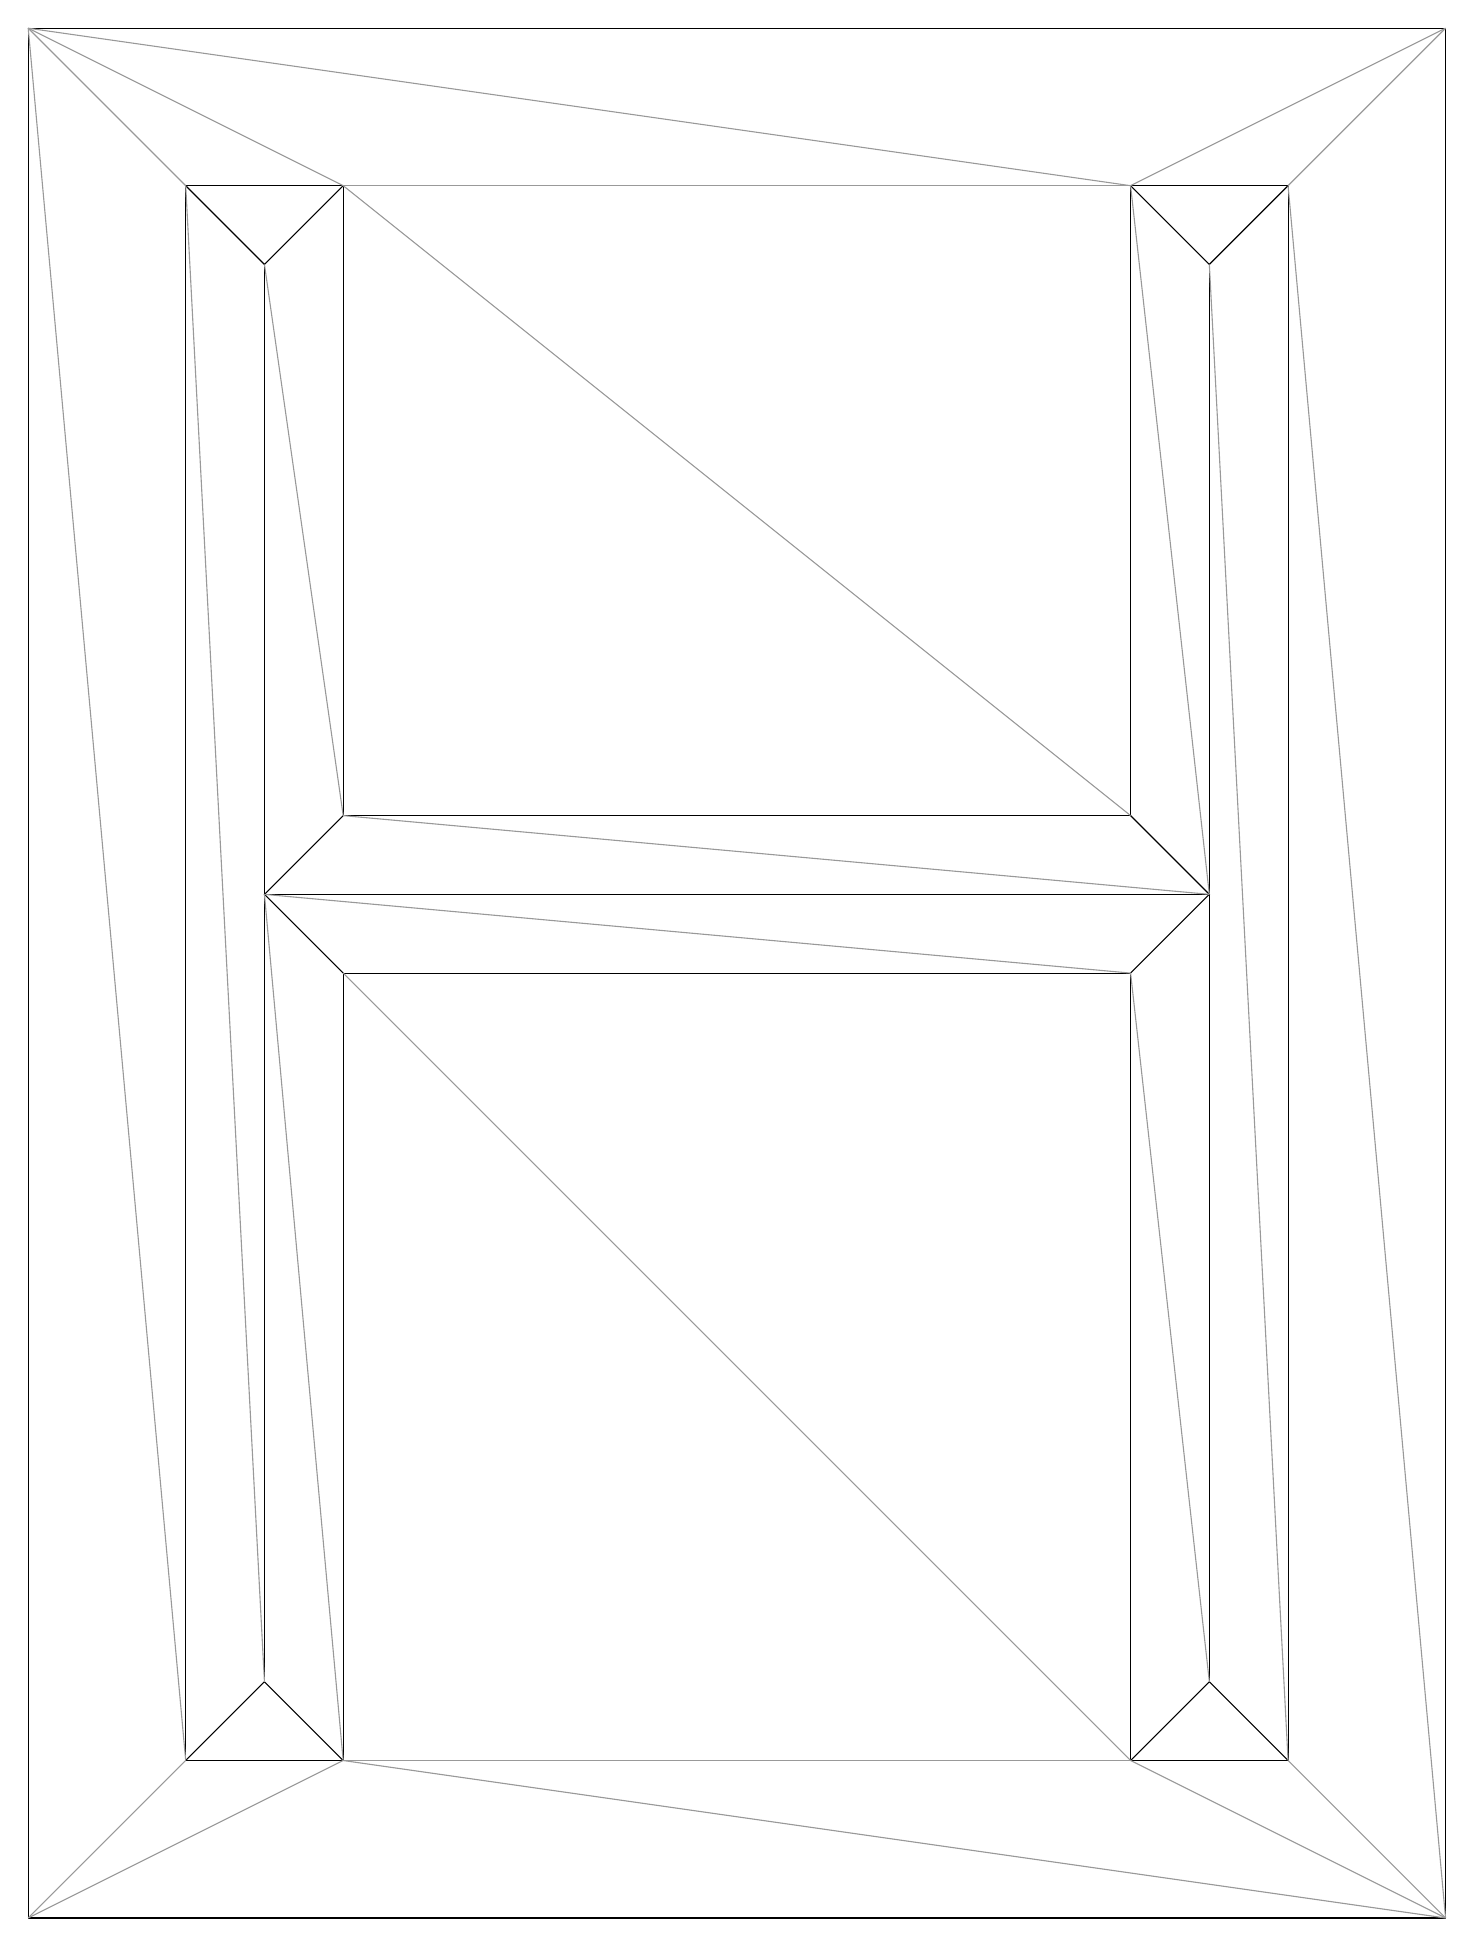
\begin{tikzpicture}
% Colors
\definecolor{outlineColor}{RGB}{0,0,0}
\definecolor{supportColor}{RGB}{153,153,153}
% Main H shape and Outline
\begin{scope}[outlineColor]
	\draw( 0, 0) % 0
	  -- ( 2, 0) % 1
	  -- ( 2,10) %12
	  -- (12,10) %13
	  -- (12, 0) % 2
	  -- (14, 0) % 3
	  -- (14,20) % 4
	  -- (12,20) % 5
	  -- (12,12) %14
	  -- ( 2,12) %15
	  -- ( 2,20) % 6
	  -- ( 0,20) % 7
	  -- cycle;  
	\draw( 0, 0) % 0
	  -- ( 1, 1) % 8
	  -- ( 2, 0);% 1
	\draw(12, 0) % 2
	  -- (13, 1) % 9
	  -- (14, 0);% 3
	\draw(14,20) % 4
	  -- (13,19) %10
	  -- (12,20);% 5
	\draw( 2,20) % 6
	  -- ( 1,19) %11
	  -- ( 0,20);% 7
	\draw( 2,10) %12
	  -- ( 1,11) %16
	  -- ( 2,12);%15
	\draw(12,10) %13
	  -- (13,11) %17
	  -- (12,12);%14
	\draw( 1, 1) % 8
	  -- ( 1,19);%11
	\draw(13, 1) % 9
	  -- (13,19);%10
	\draw( 1,11) %16
	  -- (13,11);%17
	\draw(-2,-2) %18
	  -- (16,-2) %19
	  -- (16,22) %20
	  -- (-2,22) %21
	  -- cycle;
\end{scope}
\begin{scope}[supportColor, thin]
	\draw( 0, 0) -- (-2,-2); % 0--18
	\draw( 0, 0) -- (-2,22); % 0--21
	\draw( 2, 0) -- (12, 0); % 1-- 2
	\draw( 2, 0) -- ( 1,11); % 1--16
	\draw( 2, 0) -- (-2,-2); % 1--18
	\draw( 2, 0) -- (16,-2); % 1--19
	\draw(12, 0) -- ( 2,10); % 2--12
	\draw(12, 0) -- (16,-2); % 2--19
	\draw(14, 0) -- (13,19); % 3--10
	\draw(14, 0) -- (16,-2); % 3--19
	\draw(14,20) -- (16,-2); % 4--19
	\draw(14,20) -- (16,22); % 4--20
	\draw(12,20) -- ( 2,20); % 5-- 6
	\draw(12,20) -- (13,11); % 5--17
	\draw(12,20) -- (16,22); % 5--20
	\draw(12,20) -- (-2,22); % 5--21
	\draw( 2,20) -- (12,12); % 6--14
	\draw( 2,20) -- (-2,22); % 6--21
	\draw( 0,20) -- ( 1, 1); % 7-- 8
	\draw( 0,20) -- (-2,22); % 7--21
	\draw(13, 1) -- (12,10); % 9--13
	\draw( 1,19) -- ( 2,12); %11--15
	\draw(12,10) -- ( 1,11); %13--16
	\draw( 2,12) -- (13,11); %15--17
\end{scope}
\end{tikzpicture}
}
  \label{fig:h.a}}
\subfloat[colored]{
  \includegraphics[width=0.48\linewidth]{data/h_colored.png}
  \label{fig:h.b}}
\caption[A debossed H, which contains 22 vertices and 36 faces.]{A debossed H, which contains 22 vertices and 36 faces: (a) wireframe (b) colored by the relation to its distance to an underlying plane, in RdGy colorramp~\cite[p.~???]{Brewer2003}~\cite[p.~19]{Giga17}, visualized using the GigaMesh~\cite{Mara10} framework with triangle edges rendered.}\label{fig:h}
\end{figure}

To evaluate methods available for discrete surfaces, we can increase the number of ver-
tices of our synthetic wedge using five iterations of the mid-edge subdivision scheme [PR97,
HW99].~\cite[p.~38]{Mara12}
\subsubsection{Real World Examples}
Something in Archaeology
Cuneiform Tablets
Mayan Tablets
Dynamic Earth models
Mars
Digital Terrain Models (DTMs) Mention in Mara 3.6 Summary “Dali” inspired method
Processing regular grids like Digital Terrain Models (DTMs) will gain dramatic performance increases using the estimator, while processing irregular grids with high curvatures will strongly benefit from precise computation of the volume integral invariant.~\cite[p.~143]{Mara12}
Experiment 1
Experiment 2
\section{Evaluation and Analysis}~\cite[p.~330]{Lang17}
Multi-node out of scope?!
\subsection{Timing}
%\begin{equation}
	N = input size (num. ops)
	P = processor count
	Ts(N) = Sequential execution time
	Tbest(N) = Optimal execution time
	TP(N, P) = Parallel runtime
%\end{equation}
\subsection{Speedup, efficiency}
	Speedup: 
S(N, P) = Tbest(N)/TP(N, P)

	Efficiency: 
E(N, P) = Tbest (N)/PTP(N, P) = S/P

	Costs: 
C(N, P) = PTP(N, P)
\subsection{Degree of Parallelism}
	0 < q < 1 is the sequential part
	1-q = is the parallelizable part
\subsection{Iso-efficiency}
	WK(P) = iso-efficient if it fulfills:
	TO(WK(P), P) = KWK(P)~\cite[p.~350]{Lang17}
\subsection{Scalability}
	A parallel system is called scalable only if in has an iso-efficency function
\section{Code}
Focus on theoretical work 
And specifics regarding CUDA considerations regarding its limitations
MAYBE 1 page
Dependencies
Linux vs Windows
\subsection{Integration with Legacy Code}
In order to use the full functionality of GigaMesh a batch program has to be run for generating feature vectors. These vectors contain additional information per vertex concerning surface and volume of a set of spheres intersecting the mesh. See [MKJB10] for more background information on the Multi Scale Integral Invariant (MSII) filtering technique. This operation is rather time consuming (it takes hours or even days of computing time) and therefore better runs without graphical user interface. Although generating feature vectors is quite robust against solo vertices, singularities, non-manifolds and holes, you should first clean up your mesh data to get a proper result. So switch to the advanced task of polishing your mesh in section 4.1 and return to this section when you have got a cleaned mesh. If you do not want to manipulate your mesh you may continue directly. Open a terminal and type and change to the mesh-folder by typing cd GigaMesh/mesh (note that GigaMesh stands for the GigaMesh installation folder). Then start the program 
nohup ./meshgeneratorfeaturevectors25d\_threads -f [-r 2] \& 
and use nohup at the beginning of the command and \& at the end to ensure that the job runs in the background. This is because this step can take several hours and you do not want to block the terminal.~\cite[p.~19]{Giga17}
\subsection{Distribution}
\section{Conclusions}
One I have a product and analyzed it, I can draw some conclusions.
\printindex
\listoffigures
\bibliography{thesis}{}
\bibliographystyle{plain}
\end{document}

